\section{Theory}
\label{chap:Theory}

\quad \, This project will discuss predictions using two different Neural Networks (NN) sub-classes called Recurrent Neural Network (RNN) and Long Short-Term memory cells (LSTM).\\

Typically, NNs, like MLPs or CNNs, are not proficient in handling ordered input data because they do not have a memory of the past seen data. For instance, the input data passed through the feedforward (FF), backpropagation steps, and only update the weights so that the order of the data is not relevant. Conversely, NN's recurrent classes present ways to model sequences and can remember past information, as we will study in more detail in the next sub-topics.

\subsection{Recurrent Neural Network}
\label{chap:Recurrent Neural Network}

\quad \, As we have seen from the FeedForward Neural Network (FFNN), the activation flow occurs only in one direction, from the input, passing through hidden-layers, until the output. The Recurrent Neural Network (RNN) keeps this principle but also add connections backward. In other words, in each time step (also called a frame), the RNN receives the input $x^{(t)}$ as well as the hidden-layer's activation from the previous time step $h_u^{(t-1)}$. This flow, called \textit{unrolling the network through time} \hyperref[Bib:Aurelien Geron]{[3][p. 504]} or \textit{recurrent edge in graph notation} \hyperref[Bib:Sebastian Raschka, Vahid Mirjalili]{[2][p. 744]}, is illustrated by \hyperref[Bib:Sebastian Raschka, Vahid Mirjalili]{[2][p. 744]} as follows:

\begin{figure}[H]
\label{fig:RNN1}
\centering
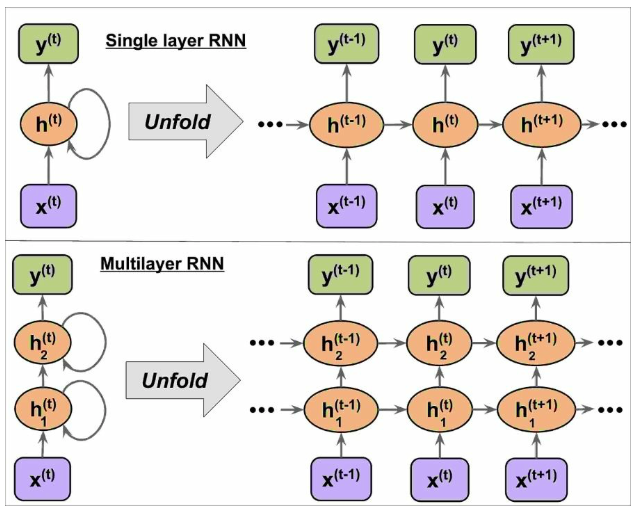
\includegraphics[height=6cm]{RNN1}
\caption{RNN's recurrent edge in graph notation for one hidden-layer and two hidden-layers.}
\end{figure}

Therefore the recurrent neuron has three sets of weights, $W_{(xh)}$ for the inputs $x^{(t)}$ and hidden-layer $h$, $W_{(hh)}$ associated with the recurrent edge, and $W_{(hy)}$ for the hidden-layer $h$ and the output layer $y^{(t)}$. The activations of the hidden units at time step $t$ is calculated by:\\

\begin{align*}
h^{(t)} &= \phi_h(z_h^{(t)}) = \phi_h(W_{xh} x^{(t)} + W_{hh} h^{(t-1)} + b_h)\\
&= \phi_h(W_h \begin{bmatrix} x^{(t)} \\ h^{(t-1)} \\ \end{bmatrix} + b_h)
\end{align*}\\

\noindent where $b_h$ is the bias vector for the hidden-unit; $z_h^{(t)}$ is the net-input; $\phi_h(.)$ is the activation function for the hidden-unit; $x^{(t)}$ is the input containing the features of the instances; $W_xh$ and $W_hh$ weights containing the connections between input and hidden-layer, and hidden-layer and hidden-layer, respectively; $W_h$ is a concatenation of $[W_{(xh)} ; W_{(hh)}]$ containing the hidden-layer's weights at time $t$ for each instance $m$ of the mini-batch.\\

Once the activation of hidden units $h^{(t)}$ is computed, the activation of output units will be:\\

$$y^{(t)} &= \phi_y(W_{hy} h^{(t)} + b_y)$$\\

\noindent where $b_y$ is the bias vector for the hidden unit and output-layer; $W_{hy}$ is the weight for the hidden-layer and output-layer.\\

Everything is summarized by the following picture from \hyperref[Bib:Sebastian Raschka, Vahid Mirjalili]{[2][p. 748]}:

\begin{figure}[H]
\label{fig:RNN3}
\centering
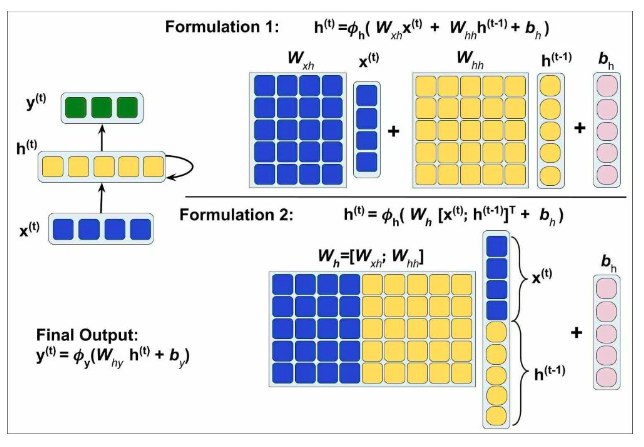
\includegraphics[height=6cm]{RNN3}
\caption{The process of computing the activations.}
\end{figure}

Hence, these recurrent neural network cells acquire a kind of memory so-called memory cells, in which there are many different applications, translated by the picture \hyperref[Bib:Aurelien Geron]{[3][p. 509]} next:

\begin{figure}[H]
\label{fig:RNN2}
\centering
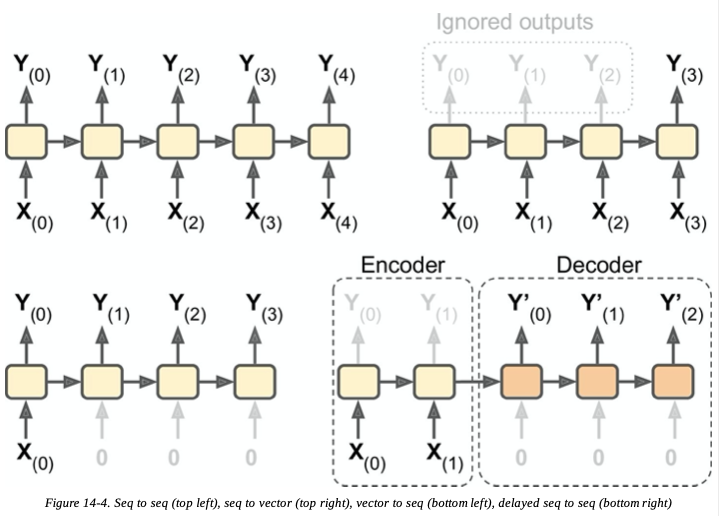
\includegraphics[height=6cm]{RNN2}
\caption{Different applications of RNN method.}
\end{figure}

The \hyperref[fig:RNN2]{picture above} shows four different applicabilities of the RNN. The first (top left) is a time series system where the inputs are values of the last N days, and the outputs are the predictions of the value shifted by one day into the future. Alternatively (top right), one could feed the RNN with a sequence of inputs and ignore all outputs except for the last one, expressing a prediction based on all previous inputs and memory cells. Conversely (bottom left), you can give a single input, and the series predictions are a function of this first input and the series of memory cells. Finally (bottom right), you can have an encoder (sequence-to-vector network) and a decoder (vector-to-sequence network) \hyperref[Bib:Aurelien Geron]{[3][p. 508]} system, in which the predictions are a function of the entire encoder and memory cells.\\

This report will apply the top left system, also called \textit{many-to-many} method \hyperref[Bib:Sebastian Raschka, Vahid Mirjalili]{[2][p. 740-1]}, where the input will be many different time series quotations (multi-features) of a given financial asset. The aim here is to predict a series of outputs to be used as a tool in a decision-making process (trading strategy).

\subsubsection{RNN's backpropagation}
\label{chap:RNN's backpropagation}

\quad \, The gradients' main idea is that the overall loss of $L$ is the sum of all loss functions from time $t=1$ to $t=T$:\\

\begin{align*}
L = \sum_{t=1}^{T}L^{(t)}
\end{align*}

\noindent and the gradients:

\begin{align*}
\frac{\partial L^{(t)}}{\partial W_{hh}}=\frac{\partial L^{(t)}}{\partial y^{(t)}} \times \frac{\partial y^{(t)}}{\partial h^{(t)}} \times ( \sum_{k=1}^{t} \frac{\partial h^{(t)}}{\partial h^{(k)}} \times \frac{\partial h^{(k)}}{\partial W_{hh}})
\end{align*}\\

\noindent and $\frac{\partial h^{(t)}}{\partial h^{(k)}}$ can be calculated by:

\begin{align*}
\frac{\partial h^{(t)}}{\partial h^{(k)}} = \prod_{i=k+1}^{t} \frac{\partial h^{(i)}}{\partial h^{(i-1)}}
\end{align*}\\

\subsubsection{Challenges of training the RNN model}
\label{chap:Challenges of training the RNN model}

\quad \, The typical RNN creates common challenges in its training process, so-called vanishing or exploding the gradients' computations, which can be explained in the figure from \hyperref[Bib:Sebastian Raschka, Vahid Mirjalili]{[2][p. 750]} below:

\begin{figure}[H]
\label{fig:RNN4}
\centering
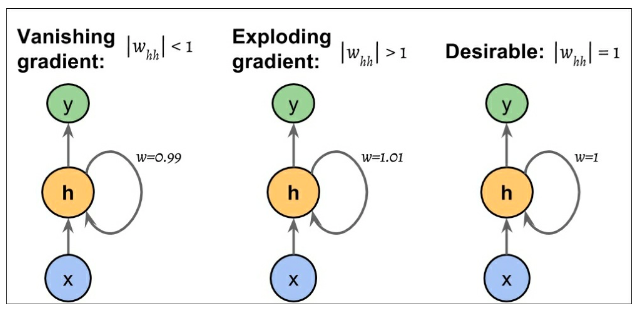
\includegraphics[height=4cm]{RNN4}
\caption{Vanishing or exploding the gradients' computations.}
\end{figure}

The multiplicative factor $\frac{\partial h^{(t)}}{\partial h^{(k)}}$ in the computation of the gradients of the loss function has $t-k$ multiplications. As a result, when $t-k$ is small, the factor $W^{(t-k)}$ becomes very small, vanishing the gradient. On the other hand, when the long-range dependencies $t-k$ is large, the factor $W^{(t-k)}$ becomes very large, exploding the gradient.\\

As we will see, the LSTM class explores some modern approaches and solutions to these challenges.

\subsection{Long Short-Term Memory Cells (LSTM)}
\label{chap:Long Short-Term Memory Cells}

\quad \, The LSTMs were introduced by \textit{Long Short-Term Memory, S. Hochreiter and J. Schmidhuber, Neural Computation, 9(8): 1735-1780, 1997}, where it was proposed a solution for the vanishing gradient problem. This method creates a building block (memory cell), giving a new representation for the hidden layer, illustrated by \hyperref[Bib:Sebastian Raschka, Vahid Mirjalili]{[2][p. 752]} as follows:

\begin{figure}[H]
\label{fig:LSTM1}
\centering
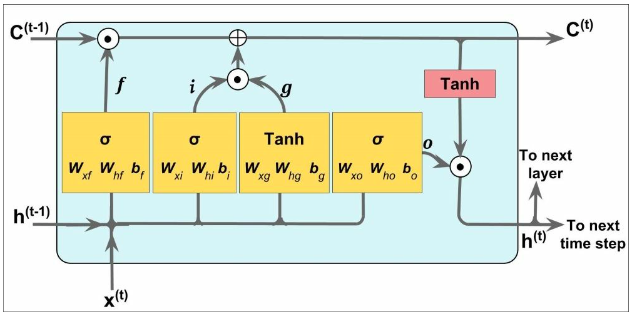
\includegraphics[height=4cm]{LSTM1}
\caption{LSTM's memory cell to avoid vanishing the gradient's computations.}
\end{figure}

First, the LSTM's cell contains four yellow boxes indicated with an activation function in the top and weights in the bottom. Each box performs a linear combination by matrix-vector multiplications on their input and weights, resulting in their output.\\

Next, this output passes through gates represented by a circle with a point in the middle ($\bigodot$ := element-wise product/multiplication \hyperref[Bib:Sebastian Raschka, Vahid Mirjalili]{[2][p. 752]}). Each of the three gates in the cell has a specific function, as follows:\\

1st.: The \textbf{forget gate} $(f_t)$ resets the cell state and decides which information passes through or suppresses. This function is defined by:\\

$$f_t = \sigma(W_{xf} x^{(t)} + W_{hf} h^{(t-1)} + b_f)$$\\

2nd.: The \textbf{input gate} $(i_t)$ and \textbf{input node} $(g_t)$ updates the cell state and is defined by:\\

$$i_t = \sigma(W_{xi} x^{(t)} + W_{hi} h^{(t-1)} + b_i)$$

\noindent and:

$$g_t = tanh(W_{xg} x^{(t)} + W_{hg} h^{(t-1)} + b_g)$$\\

3rd.: The \textbf{output gate} $(o_t)$ decides how the hidden-units updates:\\

$$o_t = \sigma(W_{xo} x^{(t)} + W_{ho} h^{(t-1)} + b_o)$$\\

Subsequently, the previous cell state $C^{(t-1)}$ is adjusted to return the current cell state $C^{(t)}$ without being directly multiplied by any weighting factor. Remark that the value compared to the RNN's recurrent edge is called cell state $C^{(t)}$ for the LSTM's models. The cell state $C^{(t)}$ is calculated as follows:\\

$$c^{(t)} = (c^{(t-1)} \bigodot f_t) \bigoplus (i_t \bigodot g_t)$$\\

\noindent where $\bigoplus$ is the element-wise-summation or addition \hyperref[Bib:Sebastian Raschka, Vahid Mirjalili]{[2][p. 753]}.\\

Hence, the hidden-units at the current time step $t$ is measured by:\\

$$h^{(t)} = o_t \bigodot tanh(c^{(t)})$$\\

\subsection{Technical Analysis}
\label{chap:Technical Analysis}

\quad Technical analysis (TA) is a tool or trading policy employed in the decision-making process in investments. Typically, TA is focused on identifying opportunities by analyzing the market's statistical metrics, including prices, volumes, and more. Besides, TA is regularly used to generate short-term trading signals, evaluating the security's strength and weakness from historical trading data.\\

Importantly, we can not mistake Technical analysis (TA) from Fundamental analysis (FA), which the latter aims to assess a security's price based on business results.\\

In this project, we will use as features or bench-mark three different TA's tools, the so-called Simple Moving Average (SMA), Exponential Moving Average (EMA), and Bollinger Bands (BB).

\subsubsection{Simple Moving Average (SMA)}
\label{chap:Simple Moving Average (SMA)}

\quad Simple Moving Average (SMA) computes the arithmetic/simple moving average of a given range of data, which could be prices, volumes, and more. In TA, SMA is widely used to indicate if financial security will continue an upward (bull) or downward (bear) trend. The formula for SMA is given by:\\

$${SMA}_t = \frac{A_1 + A_2 + ... + A_T}{T} = \frac{1}{T} \sum_{t=0}^{T} A_t$$\\

\noindent where $t = 1, 2, ..., T$ and $t \in \mathbb{N}$; $A_t$ is the value of the data stored in time series; $T$ is the number of total periods of the time series range.\\

In our GitHub repository for \href{https://github.com/fabiorodp/UiO-FYS-STK4155/tree/master/Project3}{Project3}, directory \href{https://github.com/fabiorodp/UiO-FYS-STK4155/tree/master/Project3/package/}{package/} there is a file \href{https://github.com/fabiorodp/UiO-FYS-STK4155/tree/master/Project3/package/technical_analysis.py}{technical\_analysis.py} containing a python script to return the SMA.

\subsubsection{Exponential Moving Average (EMA)}
\label{chap:Exponential Moving Average (EMA)}

\quad Exponential Moving Average (EMA) is a weighted moving average type that attributes a greater weight on the most recent data points. Thus, the EMA's reaction is more significant to recent data points than for SMA, which applies the same weight for the entire range. Although that, likely the SMA, EMA is also widely used to indicate upward (bull) or downward (bear) trends, and its formula is given by:\\

$${EMA}_t = \alpha A_t + (1 - \alpha) EMA_{(t-1)}$$\\

\noindent where $t = 1, 2, ..., T$ and $t \in \mathbb{N}$; $A_t$ is the value of the data stored in time series; $T$ is the number of total periods of the time series range; $\alpha$ is a smoothing factor given by $\alpha = \frac{2}{(T+1)}$.\\

A detail that must be stated is that the EMA tool must start from some value, and it is a protocol that its first value is an SMA.\\

In our GitHub repository for \href{https://github.com/fabiorodp/UiO-FYS-STK4155/tree/master/Project3}{Project3}, directory \href{https://github.com/fabiorodp/UiO-FYS-STK4155/tree/master/Project3/package/}{package/} there is a file \href{https://github.com/fabiorodp/UiO-FYS-STK4155/tree/master/Project3/package/technical_analysis.py}{technical\_analysis.py} containing a python script to return the EMA.

\subsubsection{Bollinger Bands (BB)}
\label{chap:Bollinger Bands (BB)}

\quad Bollinger Bands (BB) was created in the early 80s and represents a popular TA tool for finance traders. It is a measure of two standard deviations (std) away from a simple moving average (SMA) price representing overbought and oversold areas. Three lines represent the bands, the \textbf{upper band} is two std above the SMA, the \textbf{middle band} is the SMA, and the \textbf{lower band} is two std below the SMA. Typically, traders use this tool to spot sell/buy signals when the security price is above (overbought) the upper band or below (oversold) the lower bands, respectively.\\

In our GitHub repository for \href{https://github.com/fabiorodp/UiO-FYS-STK4155/tree/master/Project3}{Project3}, directory \href{https://github.com/fabiorodp/UiO-FYS-STK4155/tree/master/Project3/package/}{package/} there is a file \href{https://github.com/fabiorodp/UiO-FYS-STK4155/tree/master/Project3/package/technical_analysis.py}{technical\_analysis.py} containing a python script to return the BBs.
